% Head-Up Display
% Versión 2023
  
\subsubsection{Head Up Display }
\label{sec:HUD}
  
La simplicidad o no de presentaci\'on de la informaci\'on est\'a directamente involucrada a el número de instrumentos, por la cantidad de trabajo y secuencias de monitoreo de instrumentos que debe realizar un piloto durante las diversas fases del vuelo. En la fase crítica de aproximación y aterrizaje un piloto debe transferir su atención con mayor frecuencia de los instrumentos a las referencias fuera de la aeronave y viceversa. Un proceso de transición que lleva mucho tiempo y es fatigoso como resultado del constante reenfoque de los ojos.

Por lo tanto, se ha desarrollado un método para aliviar estos problemas en el que los datos de vuelo vitales se presentan al mismo nivel que la línea de visión del piloto cuando se ven referencias externas, es decir, cuando se mantiene una posición de ``{\it cabeza arriba}'' (head up). Los componentes de un sistema típico de visualización de esta forma, denominado \ac{HUD}, se pueden observar en la Figura \ref{fig:01.HUD} \cite{MikesFlightDeck}.

La cantidad de datos requeridos se rige por los requisitos de las diversas fases de vuelo y la función operativa de una aeronave, es decir, civil o militar, pero los  parámetros que se muestran son básicos. Los datos se transmiten desde una unidad de computadora de datos al tubo de rayos catódicos  cuya presentación es proyectada por el sistema óptico al infinito. La longitud, o rango, de las escalas está determinada por los requisitos operativos, pero normalmente solo cubren bandas estrechas de información de velocidad y altitud. Esto ayuda a reducir las marcas irrelevantes y el tiempo necesario para leer e interpretar. La  proyecci\'on óptica como una imagen simbólica compuesta sobre una placa reflectora transparente, o directamente sobre el parabrisas es lo que ve el piloto. %Se observará que la presentación de la actitud se asemeja a la de un horizonte giroscópico normal, y también que la velocidad y la altitud se presentan mediante marcadores que se registran contra escalas lineales horizontales y verticales. 

El HUD usa aplicaciones ópticas para agregar símbolos generados por computadora al campo de visión frontal del piloto, por esto se dice que es una clase de pantalla colimada, al parecer que las imágenes añadidas estan en el infinito óptico. Esto proporciona dos ventajas principales:

\begin{itemize}
\item Las imágenes permanecen alineadas con la vista exterior independientemente de cómo cambie el punto de vista del piloto.

\item El piloto no necesita volver a enfocar los ojos cuando cambia entre otro instrumento y la lectura de los datos del HUD. 
\end{itemize}

Esto significa que el sistema óptico es más complejo que un simple espejo parcialmente reflectante.

Una lente esférica, plano-convexa colimará una imagen, pero este enfoque tan simple tiene algunas deficiencias: introducirá distorsión geométrica en la imagen, no todos los colores estarán enfocados para la misma posición de la lente y cuando el centro de la imagen esté enfocado, los bordes de la imagen no lo estarán.

Se emplean lentes esféricos a pesar de estas limitaciones porque se pueden hacer formas esféricas con gran precisión con costos moderados. Las lentes asféricas fabricadas con una precisión similar pueden tener propiedades ópticas sustancialmente mejores, pero las complejidades de fabricación pueden hacer que el costo sea prohibitivo.

De todas maneras las lentes asféricas no son la respuesta final porque sólo pueden corregir distorsiones geométricas, puesto que las lentes, esféricas o no, funcionan refractando la luz y los ángulos de refracción cambian con la longitud de onda de ésta. Las lentes asféricas están sujetas a la aberración cromática al igual que las lentes esféricas.

El conjunto de óptica de colimación HUD consta de varias lentes simples. Al menos una de las lentes estará hecha de un material con un índice de refracción diferente. Las lentes individuales y los materiales de las lentes se eligen de modo que las aberraciones de las lentes individuales tiendan a cancelarse, dando como resultado una lente compuesta que tiene un rendimiento superior al de sus componentes.

Combinadores

Parcialmente reflectante

Los combinadores vienen en varias variedades. Uno simple es un espejo plano parcialmente plateado. Es viable pero pierde luz. Si tiene una relación de transmisión del 50\%, la mitad pasa y la otra mitad se refleja. Esto no es un problema para los datos de HUD, ya que la fuente de HUD se puede hacer más brillante. Sin embargo, es un problema con respecto a la visión delantera del piloto. La mitad de eso también se refleja. Puede jugar con la relación de transmisión para reducir la pérdida de visión hacia adelante, pero eso solo funciona hasta ahora.

Otra característica molesta de estos combinadores es la presencia de reflejos internos. La luz se reflejará en las superficies delantera y trasera. Los reflejos aparecen como imágenes fantasma.

Los reflejos internos se pueden minimizar utilizando un revestimiento antirreflectante en la superficie no reflectante del sustrato del espejo. El recubrimiento genera reflejos en sus superficies frontal y posterior. El grosor del recubrimiento se controla de modo que la reflexión de la superficie posterior esté desfasada con la reflexión de la superficie frontal. Al estar fuera de fase, se anulan entre sí. El índice de refracción se elige de manera que las dos reflexiones sean de la misma magnitud para asegurar la mejor cancelación. Los revestimientos antirreflectantes se ajustan a una sola longitud de onda de luz, pero dan resultados adecuados en una gama de colores.

Dicroico

Un combinador mejorado hace uso de un espejo dicroico. Esto es similar a un recubrimiento antirreflectante, pero se utilizan muchas capas y el grosor del recubrimiento se elige para mejorar el reflejo de una longitud de onda particular. Otras longitudes de onda pasan con atenuación mínima. Cuando se usa un espejo dicroico, una banda estrecha de colores se bloquea fuera de la vista frontal del piloto y se reemplaza por los datos del HUD. Debido a que el color de la pantalla HUD coincide con la característica dicroica, prácticamente toda la luz generada por HUD se dirige al piloto y solo se bloquea una pequeña cantidad de luz exterior. Un combinador dicroico también está sujeto a reflexiones internas. Se utiliza un revestimiento antirreflectante en la parte trasera del combinador para controlar esto.

Catadióptrico

El combinador no tiene que ser plano. Se puede usar un combinador curvo para implementar parte de toda la colimación. Esto generalmente se conoce como HUD catadióptrico. Catadióptrico se refiere a un sistema óptico que incorpora elementos reflectantes y refractivos. Una gran ventaja de las ópticas reflectantes es que no sufren aberración cromática. Al igual que las lentes, se fabrican más fácilmente en formas esféricas y, por lo tanto, también sufren de aberración esférica. Esto se puede corregir a través del diseño del sistema óptico tal como se corrige un sistema basado en lentes.

Holográfico

El término ``{\em HUD holográfico}'' puede recordar a una película de SciFi pero, lLa realidad es mucho simple. Un HUD holográfico simplemente usa un elemento óptico holográfico o HOE como combinador. Esta es una rejilla de difracción especializada que puede combinar y colimar. Los HOE pueden tener una longitud de onda muy específica para permitir que la cantidad máxima de luz del campo de visión delantero pase al piloto. Un HUD holográfico puede ofrecer un campo de visión más amplio para un peso dado que un HUD basado únicamente en lentes y/o espejos.


\begin{figure}[!htb]
  \centering
  \subfigure[Principio de funcionamiento del
  HUD ]{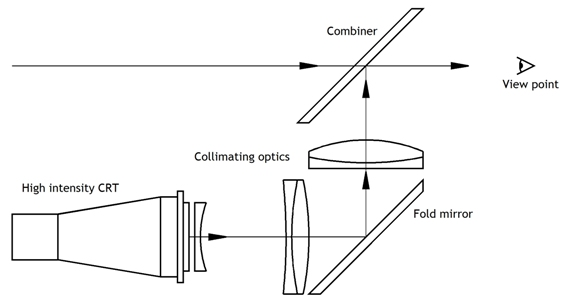
\includegraphics[width=0.45\textwidth]{01.tablero.instrumentos/U01.imagenes/1.2.clasificacion.instrumentos/hud_esquema.jpg}}
  \subfigure[Vista de un
  HUD]{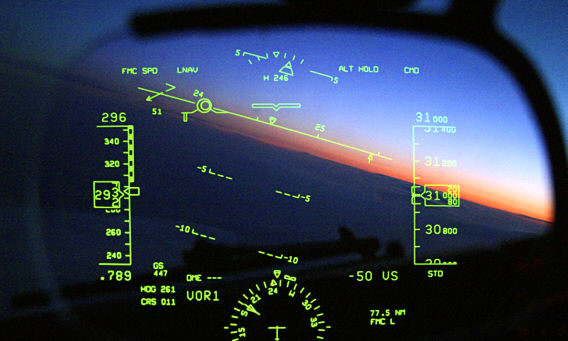
\includegraphics[width=0.45\textwidth]{01.tablero.instrumentos/U01.imagenes/1.2.clasificacion.instrumentos/hud.jpg}}
  
  \caption{HUD}
\label{fig:01.HUD}
\end{figure}


\begin{tcolorbox}
Un video interesante que cuenta la historia del HUD se encuentra en el siguiente link: 

  {
\includegraphics[width=0.1\textwidth]{01.tablero.instrumentos/U01.imagenes/Video.png}}\,
\href{https://www.youtube.com/watch?v=ypIbmfm7n8A}{The Evolution of the Head-Up Display}.
\vspace{3mm}


  Existen en el mercado peque\~nos \ac{HUD} para uso en aviaci\'on general como el provisto por la empresa Thales, el 
\href{https://www.thalesgroup.com/en/markets/aerospace/flight-deck-avionics-equipment-functions/topmax-wearable-hud-commercial-aircraft}{TopMax}.
\end{tcolorbox}


Tambi\'en se han desarrollado los \ac{EFVS} que son sistemas de visi\'on sint\'eticos, ver Figura \ref{fig:01.efvs}, 
 que proporciona una imagen de la escena y la muestra al piloto con el fin de proporcionar una imagen en la que la escena y los objetos en ella se pueden detectar mejor, esto es, un EFVS es un sistema que proporciona al piloto una imagen mejor que la visión humana sin ayuda. 

Los EFVS incluyen sensores de imágenes como una cámara a color, una cámara de infrarrojos o un radar y, normalmente una pantalla para el piloto, que puede ser una pantalla montada en la cabeza del mismo o una pantalla frontal. Un EFVS se puede combinar con un sistema de visión sintético para crear un sistema de visión combinado.
\href{https://www.youtube.com/watch?v=phbZintCgVA}{Video de un HUD/EFVS}.

\begin{figure}[!htb]
  \centering
\subfigure[EFVS]{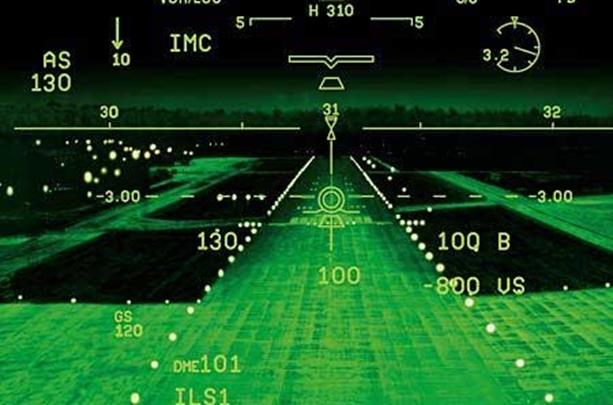
\includegraphics[width=0.45\textwidth]{01.tablero.instrumentos/U01.imagenes/1.2.clasificacion.instrumentos/EFVS_Photo.jpg}}
\subfigure[EFVS]{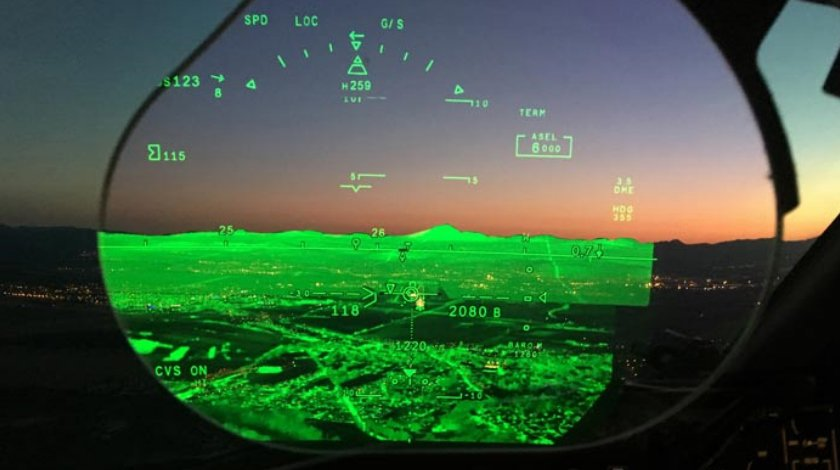
\includegraphics[width=0.45\textwidth]{01.tablero.instrumentos/U01.imagenes/1.2.clasificacion.instrumentos/efvs.jpg}}
  
  \caption{EFVS}
\label{fig:01.efvs}
\end{figure}


